\documentclass{article}%
\usepackage[T1]{fontenc}%
\usepackage[utf8]{inputenc}%
\usepackage{lmodern}%
\usepackage{textcomp}%
\usepackage{lastpage}%
\usepackage[head=40pt,margin=0.5in,bottom=0.6in]{geometry}%
\usepackage{graphicx}%
%
\title{\textbf{ELN y disidencias de la FARC intentan reclutar venezolanos}}%
\author{El Nacional Web}%
\date{16/10/2018}%
%
\begin{document}%
\normalsize%
\maketitle%
\textbf{URL: }%
http://www.el{-}nacional.com/noticias/latinoamerica/eln{-}disidencias{-}farc{-}intentan{-}reclutar{-}venezolanos\_256059\newline%
%
\textbf{Periodico: }%
EN, %
ID: %
256059, %
Seccion: %
Latinoamérica\newline%
%
\textbf{Palabras Claves: }%
Mundo, Colombia, Latinoamérica\newline%
%
\textbf{Derecho: }%
CONTEXTO, %
Otros Derechos: %
, %
Sub Derechos: %
\newline%
%
\textbf{EP: }%
NO\newline%
\newline%
%
\textbf{\textit{Juan Carlos Ortega, analista del conflicto armado, alega que una de las razones para que estos grupos busquen personal en las fronteras es la declaratoria de guerra del gobierno a las disidencias y el cese temporal de la mesa de diálogos con el ELN}}%
\newline%
\newline%
%
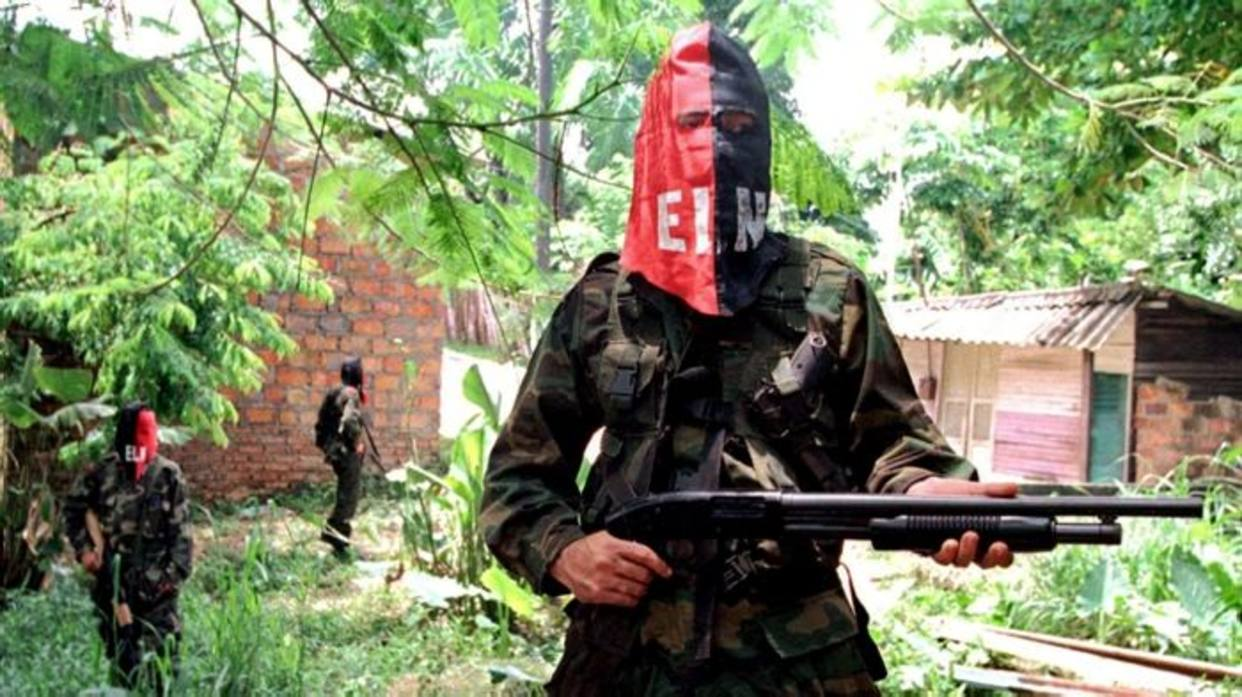
\includegraphics[width=300px]{177.jpg}%
\newline%
%
El Ejército de Liberación Nacional (ELN) y disidencias de las Fuerzas Armadas Revolucionarias de Colombia (FARC) intentan reclutar a venezolanos con promesas de empleo rentable para subsanar carencias de la crisis venezolana o, en algunos casos, bajo amenaza.%
\newline%
%
Helder Giraldo, comandante de la Octava División del Ejército Nacional, informó que su unidad militar tiene casos concretos~“de reclutamiento de ciudadanos del vecino país en las filas de los diferentes grupos armados organizados que delinquen en los departamentos limítrofes como los son el frente Domingo Láin Sáenz del Eln, y el GAO (disidencias) con las subestructuras del 1 y el 28 (antiguos frentes de Farc)”, reseñó~La Opinión.%
\newline%
%
El alto mando militar de Colombia indicó que tienen 27 casos registrados por las autoridades en los últimos meses como evidencia de la participación de venezolanos capturados cuando cometían delitos de extorsión,~tráfico de estupefacientes y tráfico de armas y municiones, y de otros que murieron en combates con soldados.%
\newline%
%
Juan Carlos Ortega, analista del conflicto armado, alega que una de las razones para que estos grupos busquen personal en las fronteras es la declaratoria de guerra del gobierno a las disidencias y el cese temporal de la mesa de diálogos con el ELN.%
\newline%
%
“El cerco militar que se les ha venido cerrando no permite que interactúen tanto con la gente de municipios del interior, además, la porosidad de la frontera, con la aquiescencia del gobierno venezolano, es el caldo de cultivo perfecto para que estos grupos busquen fortalecerse en zona frontera”, explica~el especialista.%
\newline%
%
Con información de~La Opinión%
\newline%
%
\end{document}